\chapter{Background and related work}

In this chapter, the background and fundamentals related to this thesis
\section{Stereotypes, language and stereotyping}
\subsection{Background}

Traditionally, there have been two kinds of cognitive processes called intuition and reason \cite{kahneman2002representativeness}. Dual process is the general label adopted where in two cognitive operations are described with generic labels "system 1" and "system 2" \cite{kahneman2002representativeness}. System 1 describes the cognitive mode, which is intuitive and fast. System 2 on the other hand is reflective  controlled. Table \ref{tab:cognitive systems} gives an overview of the two systems. These two cognitive modes play a role in the formation of bias. Biases in the cognition arises due to the attribute substitution. Attribute substitution heuristics states that "when confronted with a difficult question, people often answer an easier one instead, usually
without being aware of the substitution" \cite{kahneman2002representativeness}. Simply put, the target attribute (difficult question) is substituted by a representative and available heuristic attribute (simple question that resembles the difficult question). This substitution leads to systematic biases. This implicit/systematic biases are formed by the system - 1 due to its fast, automatic and associative characteristic feature \cite{kahneman2002representativeness}. "System 1 generate impressions of the attributes of objects of perception and thought"\cite{kahneman2003maps}. The "impressions that are similar, especially if a label is attached, tend to cohere into categories(generalization, concepts)"\cite{fiske1998stereotyping}. Categorization leads to generalization of group behavior, expectancies. The overgeneralized beliefs and expectancies about a category or group of people refers to stereotypes \cite{allport1954nature}\cite{fiske1998stereotyping}. 
% This cognitive representation with noisy false attribute leads to prejudice (emotion). Judging with stereotypical beliefs and  prejudicial attitude results in discrimination.

% Please add the following required packages to your document preamble:
% \usepackage{booktabs}
% \usepackage{graphicx}
\begin{table}[]
\centering
\scalebox{0.5}{
\resizebox{\columnwidth}{!}{%
\begin{tabular}{@{}ll@{}}
\toprule
System 1 (Intuitive)                  & System 2 (Reflective)              \\ \midrule
\multicolumn{1}{|l|}{Do not require working memory} & \multicolumn{1}{l|}{Requires working memory} \\ \midrule
\multicolumn{1}{|l|}{Autonomous}      & \multicolumn{1}{l|}{Controlled}    \\ \midrule
\multicolumn{1}{|l|}{Rapid, Parallel} & \multicolumn{1}{l|}{Slow, serial}  \\ \midrule
\multicolumn{1}{|l|}{Associative}     & \multicolumn{1}{l|}{Rule governed} \\ \bottomrule
\end{tabular}%
}}
\caption{Two cognitive systems }
\label{tab:cognitive systems}
\end{table}

\pagebreak
% \begin{itemize}
%     \item Origin of bias (System -1 and system -2) ; TWO FAMILIES OF COGNITIVE OPERATIONS \cite{kahneman2002representativeness}
%     \item  How stereotypes are inevitably formed (implicit bias) ??
%     Impressions + labels ...
%     \cite{fiske1998stereotyping}
%     \item Difference between stereotype and prejudice \cite{fiske1998stereotyping}
%     \begin{itemize}
%         \item Stereotype (Cognitive) : An overgeneralized belief about a particualr group of people.This need not be negative but sometimes be accurate, like Lions have four legs. But the problem arises if the stereotype is rooted with inaccurate association formed between target from social groups (gender, ethnicity ..) and its attribute. 
%         \item Prejudice (Attitude) : "pre-judgement", typically negative attitude towards an individual or group.
%         \item Discrimination (Behaviour) : Stereotypical beliefs combined with prejudicial attitude towards social groups can drive the behavior to change which results in discrimination.\label{crashcrouse}\footnote {\url{https://www.youtube.com/watch?v=7P0iP2Zm6a4&ab_channel=CrashCourse}}
%     \end{itemize}
% \end{itemize}
\subsection{Perspectives of stereotypes}
A lot of research has been carried out on stereotype from as early as 1927 with evolving definitions and constructs being put forth by investigators. This section defines the different perspectives of stereotype and finally the perspective used in this thesis.
\\
\\
As can be seen in the table \ref{tab:stereotype_taxonomy} taken from "meaning of stereotype" in psychology
\cite{ashmore1981conceptual}, there are many perspectives concerning stereotypes. Every definition deal with a dimension of stereotype  such as "fixed, rigid", "generalization","incorrect" etc. \cite{kanahara2006review} describes that each definition belongs to combination of components ("adjectives" and "nouns") such as "superficial", "characteristic", "fixed", "image", "impression", "belief", "ethnic", "cultural" etc.  The definitions include "incorrect beliefs" \cite{katz1935racial}, "the attribution of general psychological characteristics to large human groups" \cite{watson1974psychology}, "an inaccurate, rigid, and oversimplified image of members of a social
group, especially an out group" \cite{coon1994essentials} among others. 
Among the definitions seen in the table \ref{tab:stereotype_taxonomy} and the ones stated above, the common component or dimension is "group concept (generalized)" and "beliefs".  \cite{kanahara2006review} uses these two components and posits that "stereotype is a belief about a group of individuals"  \cite{kanahara2006review}.
considering an example, "Japanese do karate"; according to the \cite{kanahara2006review}, this is a stereotype as it involves a belief (do karate) about an entire group (Japanese). "Stereotypes can be positive or negative, correct or incorrect, simple or complicated, as beliefs can be positive or negative." \cite{kanahara2006review}. According to \cite{kanahara2006review}, the beliefs about a group of people cannot be completely validated to be true.
These stereotypical beliefs, when instantiated, lead to stereotypic expectancies (stereotyping). Considering the same stereotype, "Japanese do karate", the application of this stereotype would be to judge a Japanese person by saying, "ken must do karate, because he is a Japanese".
Until this point, stereotypes can be understood as generalized beliefs about a group of individuals, and stereotyping is generalized expectancies based on the belief. 

\\
\\
"Stereotypes are considered to be the "pictures in the head" of individuals looking out into their social worlds"\cite{macrae1996stereotypes}. Hence, one perspective is that of the generalized impressions people have in their head. On the other hand, these generalized impressions could be shared socially among the ethnic or cultural groups. This gives a socially shared perspectives of stereotypes. "Stereotypes only have meaning to the extent they are socially shared. But stereotypes only have meaning to the extent they are socially shared"\cite{macrae1996stereotypes}. Putting all together, stereotypes are generalized beliefs about a group of individuals. These beliefs could be "pictures in the head" or it could be socially shared. Considering the perspective that socially shared stereotypes only have meaning, there arises a need for a medium for the transmission of stereotypes. Language thus plays an important role in the sustenance and maintenance of stereotypes\cite{macrae1996stereotypes}.



% \begin{itemize}
%         \item Stereotypes cannot be avoided, as they are implicitly formed as a part of the cognitive process. When these associations/ implicit bias (deviation from rationality) are overgeneralized followed by, this leads to stereotyping. Hence arises two perspectives or dimensions of stereotypes 
%             \begin{itemize}
%                 \item Stereotypes (as pictures in head / Implicit associations)
%                 \item Stereotyping (Socially shared Stereotypical associations / Overgeneralized beliefs and expectancies) 
%             \end{itemize}
%             \item Coming to this thesis, social stereotypes are being studied where the focus is mainly on examining 
%             \begin{itemize}
%                 \item Biased stereotypical associations
%                 \item Socially shared Stereotypes
%             \end{itemize}
% \end{itemize}
% \begin{itemize}
%     \item Describe two perspective, Stereotypes as pictures in head and stereotyping (shared social beliefs and expectancies)
%     \item Definitions of stereotype from other papers
%         \begin{itemize}
%             \item Stereotypes definition taxonomy \cite{ashmore1981conceptual}
%         \end{itemize}
%     \item Cognitive processes in stereotyping and intergroup behavior \cite{hamilton2015cognitive}
%     \item Stereotypes and stereotyping \cite{macrae1996stereotypes}
%     \item Prescriptive and descriptive stereotyping
%     \item Types of harms caused by bias [Kate Crawford. 2017. The Trouble with Bias. Keynote
% at NeurIPS]
% \end{itemize}
\subsection{Contribution of language}

The role of language in maintenance of social category stereotypes has been significant\cite{burgers2020language}.
 Social categories and Stereotypes Communication (SCSC) \cite{beukeboom2019stereotypes} mentions two broad linguistic biases, namely, linguistic labels used to refer to categorized individuals. Out of generic and specific labels all, Generic labels play a crucial role in stereotype communication\cite{burgers2020language}. Generic labels refer to a category as a whole, e.g.("women are ...") while specific labels refer to subgroups ("Young women.."). Typically, generic labels facilitate the communication of stereotypic information when compared to specific labels\cite{burgers2020language}. 
 
 The second group of linguistic biases in stereotype communication relates to the language use in communication\cite{beukeboom2019stereotypes}. It has been shown that speakers systematically vary the language when either describing the stereotypical consistent behavior or stereotypical inconsistent behavior. The stereotypic consistent behavior is described with high essentialism  \cite{burgers2020language}.  
    \begin{itemize}
        \item Stereotypes as collective belief systems \cite{macrae1996stereotypes}
        \item How language contributes to stereotype formation \cite{burgers2020language}
        \item How stereotypes are shared through language: a
    review and introduction of the social categories
    and stereotypes communication (SCSC) framework \cite{beukeboom2019stereotypes}
    \end{itemize}
    % \pagebreak

% Please add the following required packages to your document preamble:
% \usepackage{booktabs}
% \usepackage{graphicx}
% \usepackage{lscape}
\begin{landscape}
\begin{table}[]
\centering
\resizebox{\columnwidth}{!}{%
\begin{tabular}{@{}cllcll@{}}
\toprule
\multicolumn{3}{c}{Stereotype not defined as bad, but it is a} &
  \multicolumn{3}{c}{Stereotype defined as bad generalization/category/concept; due to} \\ \midrule
\multicolumn{1}{|c|}{Generalization} &
  \multicolumn{1}{l|}{Category/concept} &
  \multicolumn{1}{l|}{Incorrectly learned} &
  \multicolumn{1}{c|}{Overgeneralized} &
  \multicolumn{1}{l|}{Factually incorrect} &
  \multicolumn{1}{l|}{Rigid} \\ \midrule
\begin{tabular}[c]{@{}c@{}}"Stereotyping may be defined as the tendency to attribute \\ generalized and simplified characteristics to group of people "\end{tabular} &
  \begin{tabular}[c]{@{}l@{}}"A stereotype is a commonly thought of \\ as a categorical response, i.e. membership  is \\ sufficient to evoke that the stimulus person\\  possess all the attributes belonging to that category"\end{tabular} &
  \begin{tabular}[c]{@{}l@{}}"Unlike other generalization ...\\  stereotypes are based on rumors, \\ anecdotes in short on evidence which \\ is insufficient to justify the generalization\end{tabular} &
  ".. a stereotype is an exaggerated belief associated with a category" &
  \begin{tabular}[c]{@{}l@{}}" A stereotype is a fixed impression, which confirms \\ very little to the fact it pretends to represent"\end{tabular} &
  "Stereotype .. the disposition to think in rigid categories" \\ \bottomrule
\end{tabular}%
}
\caption{A taxonomy of psychological meaning of the contract "stereotype" derived from Brigham's (1971) Analysis }
\label{tab:stereotype_taxonomy}
\end{table}
\end{landscape}

\section{Machine learning and deep learning}
\subsection{Machine learning pipeline}
    \begin{itemize}
        \item Machine learning setup by abu mustafa 
        \begin{figure}[t]
            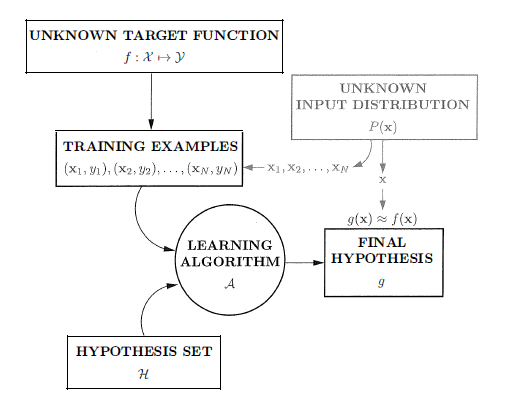
\includegraphics[width=8cm]{thesis/figures/Learning problem.PNG}
            \centering
            \caption{The learning problem setup}
            \label{fig:The learning problem setup}
        \end{figure}
        \begin{enumerate}
            \item Explain different components of learning problem  learning problem 
            
        \end{enumerate}
        \item Types of training (supervised, unsupervised, reinforcement learning and focus on supervised)
        \item Learning models (Classification, regression)
        \item Linear and logistic Regression and gradient descent 
        \textbf{Refer to udemy machine learning course notes}
        % \item SVM and selected classifiers \textbf{TBD ??}
    \end{itemize}
\subsection{Neural Networks architecture}
    \begin{itemize}
        \item Deep learning vs Machine learning 
        \item Neural network basic setup (perceptron learning algorithm)
        \item Basic neural network forward pass and backward pass
        \item  Deep neural network and its variants
        \item Refer \url{https://github.com/mvdheram/DeepLearning-Notebooks/blob/main/Introduction_to_PyTorch.ipynb}
        \item \textbf{IMP : Classification using neural networks} 
    % \end{itemize}
    % \begin{itemize}
        \item Dropout for regularization 
    \end{itemize}
\subsection { Recurrent Neural Networks }
            \begin{itemize}
                \item Limitations of NN 
                \item Why RNN when dealing with text ?
                \item Contextual word embedding
            \end{itemize}

\subsection{Transformer architecture}
    
\section{Natural language processing and language modeling}
    \textbf{Text classification algorithms : a survey }\url{https://www.mdpi.com/2078-2489/10/4/150/htm}
    \subsection{Vector representation of text}
    \begin{itemize}
        \item What is NLP?
        \item Feature vectors for text 
            \begin{itemize}
                \item Bag of words
                \item TF-IDF
            \end{itemize}
        \item Word embeddings
        \item Static word embedding
        \item Word2vec, glove basic architecture
    \subsection{Text classification}    \item Text classification 
        \begin{itemize}
            \item classification types (Binary, multi class, multi label)
            \item LPP
            \item Sigmoid activation function and binary cross entropy loss function
            \item General text classification metrics (Accuracy, precision, recall, fmeasure)
            \item Multi label text classification and problem transformation 
        \end{itemize}
    \end{itemize}
    \subsection{Language modeling}
    \subsection{Transfer learning}
    \subsection{BERT architecture}
% \section {Evaluation metrics}    
\section{Bias and social bias in Natural language processing}
\begin{itemize}
    \item A critical survey of bias in NLP \cite{blodgett2020language}
    \item A survey on Bias in Deep NLP \cite{garrido2021survey}
\end{itemize}